%%%%%%%%%%%%%%%%%%%%%%%%%%%%%%%%%%%%%%%%%
% Beamer Presentation
% LaTeX Template
% Version 1.0 (10/11/12)
%
% This template has been downloaded from:
% http://www.LaTeXTemplates.com
%
% License:
% CC BY-NC-SA 3.0 (http://creativecommons.org/licenses/by-nc-sa/3.0/)
%
%%%%%%%%%%%%%%%%%%%%%%%%%%%%%%%%%%%%%%%%%

%----------------------------------------------------------------------------------------
%	PACKAGES AND THEMES
%----------------------------------------------------------------------------------------

\documentclass{beamer}

\mode<presentation> {

% The Beamer class comes with a number of default slide themes
% which change the colors and layouts of slides. Below this is a list
% of all the themes, uncomment each in turn to see what they look like.

%\usetheme{default}
%\usetheme{AnnArbor}
%\usetheme{Antibes}
%\usetheme{Bergen}
%\usetheme{Berkeley}
%\usetheme{Berlin}
%\usetheme{Boadilla}
%\usetheme{CambridgeUS}
%\usetheme{Copenhagen}
%\usetheme{Darmstadt}
%\usetheme{Dresden}
%\usetheme{Frankfurt}
%\usetheme{Goettingen}
%\usetheme{Hannover}
%\usetheme{Ilmenau}
%\usetheme{JuanLesPins}
%\usetheme{Luebeck}
%\usetheme{Madrid}
%\usetheme{Malmoe}
%\usetheme{Marburg}
%\usetheme{Montpellier}
%\usetheme{PaloAlto}
%\usetheme{Pittsburgh}
%\usetheme{Rochester}
%\usetheme{Singapore}
%\usetheme{Szeged}
%\usetheme{Warsaw}
\usetheme{Amsterdam}

% As well as themes, the Beamer class has a number of color themes
% for any slide theme. Uncomment each of these in turn to see how it
% changes the colors of your current slide theme.

%\usecolortheme{albatross}
%\usecolortheme{beaver}
%\usecolortheme{beetle}
%\usecolortheme{crane}
%\usecolortheme{dolphin}
%\usecolortheme{dove}
%\usecolortheme{fly}
%\usecolortheme{lily}
%\usecolortheme{orchid}
%\usecolortheme{rose}
%\usecolortheme{seagull}
%\usecolortheme{seahorse}
%\usecolortheme{whale}
%\usecolortheme{wolverine}

%\setbeamertemplate{footline} % To remove the footer line in all slides uncomment this line
%\setbeamertemplate{footline}[page number] % To replace the footer line in all slides with a simple slide count uncomment this line

%\setbeamertemplate{navigation symbols}{} % To remove the navigation symbols from the bottom of all slides uncomment this line
}

\usepackage{graphicx} % Allows including images
\usepackage{booktabs} % Allows the use of \toprule, \midrule and \bottomrule in tables
\usepackage[utf8]{inputenc}
% http://tex.stackexchange.com/questions/107637/repeated-division-converting-from-base-10-to-another-base


\newcount\total
\newcount\lasttotal
\newcount\targetbase

\def\digittoalpha#1{%
    \ifcase#1\relax0\or1\or2\or3\or4\or5\or6\or7\or8\or9%
    \or a\or b\or c\or d\or e\or f\or g\or h\or i\or j\or k\or l\or m%
    \or n\or p\or p\or q\or r\or s\or t\or u\or v\or w\or x\or y\or z\else?\fi%
}

\def\baseconversiontable#1#2{%
    \begin{tikzpicture}[every node/.style={minimum width=1cm, minimum height=0.5cm}, x=1cm,y=0.5cm]
    %
    \total=#1%
    \targetbase=#2
    \def\newnumber{}
    %
    \pgfmathloop
    \ifnum\total<1
    \else
        %
        \ifnum\pgfmathcounter>1
            \node at (\pgfmathcounter, -\pgfmathcounter+1) (tmp) {\the\targetbase};
            \draw (tmp.north west) |- (tmp.south east);
            %
            \node at (\pgfmathcounter-1, -\pgfmathcounter) (tmp) {\pgfmathparse{int(-\total*\targetbase)}\pgfmathresult};
            \draw (tmp.south west) -- (tmp.south east);
            %
            \pgfmathparse{int(\lasttotal-\total*\targetbase)}%
            \let\digit=\pgfmathresult
            \node at (\pgfmathcounter-1, -\pgfmathcounter-1) [text=red] {\digit};
            \edef\newnumber{\digit\newnumber}
        \fi
        %
        \ifnum\total<\targetbase
            \edef\currentdigit{\uppercase{\digittoalpha{\the\total}}}%
            \edef\newnumber{\currentdigit\newnumber}
            \ifnum\total>9
              \edef\currentdigit{\noexpand\rm{\currentdigit}}%
            \fi
            \node at (\pgfmathcounter, -\pgfmathcounter) [text=red]  {\the\total};
            %\color{black}\the\total(\color{red}\currentdigit\color{black})
            %};
        \else
            \node at (\pgfmathcounter, -\pgfmathcounter) {\the\total};
        \fi
        \lasttotal=\total
        \divide\total by\targetbase
    \repeatpgfmathloop    
    \draw [->] (\pgfmathcounter-1,-\pgfmathcounter-1) -- ++(-0.5,0); 
    %\node [anchor=west] at (1, -\pgfmathcounter-2) {$#1=\newnumber_{\the\targetbase}$};
    \end{tikzpicture}   
}



\usepackage{framed}

\usepackage{algorithm}
\usepackage[noend]{algpseudocode}
\definecolor{algocoul}{rgb}{0,0,0.75}
\definecolor{algocom}{rgb}{.75,.25,0}
\floatname{algorithm}{Algorithme}

\usepackage{tikz}
\usepackage{tikz-timing}
\usepackage{tkz-graph} 
\usetikzlibrary{arrows,shapes.gates.logic.US,shapes.gates.logic.IEC,calc,shapes.geometric,positioning}
\tikzset{
  multiplexer/.style={
    draw,
    trapezium,
    shape border uses incircle, 
    shape border rotate=270,
    minimum size=18pt
  }  
}

\tikzset{
    alu/.style={trapezium,
            trapezium angle=26,
            shape border rotate=180,
            minimum width=3cm,
            minimum height=2cm,
            trapezium stretches=true,
            append after command={%
                    \pgfextra
                        \draw (\tikzlastnode.top left corner) --
                           (\tikzlastnode.top right corner) -- 
                           (\tikzlastnode.bottom right corner) -- 
                           ($(\tikzlastnode.bottom right corner)!.666!(\tikzlastnode.bottom side)$)--
                           ([yshift=-1cm]\tikzlastnode.bottom side)--
                           ($(\tikzlastnode.bottom side)!.334!(\tikzlastnode.bottom left corner)$)--
                           (\tikzlastnode.bottom left corner)--
                           (\tikzlastnode.top left corner);
                    \endpgfextra}},
}




\usepackage[europeanresistors, siunitx]{circuitikz}
\usepackage{eurosym}
\usepackage{listings}

%----------------------------------------------------------------------------------------
%	TITLE PAGE
%----------------------------------------------------------------------------------------

\title[Architecture]{Architecture des ordinateurs} % The short title appears at the bottom of every slide, the full title is only on the title page

\author{Jérémy Fix} % Your name
\institute[CS] % Your institution as it will appear on the bottom of every slide, may be shorthand to save space
{
CentraleSupélec \\ % Your institution for the title page
\medskip
\textit{jeremy.fix@centralesupelec.fr} % Your email address
}
\date{2017-2018} % Date, can be changed to a custom date

\begin{document}

\begin{frame}
\titlepage % Print the title page as the first slide
\end{frame}

%% \begin{frame}
%% \frametitle{Overview} % Table of contents slide, comment this block out to remove it
%% \tableofcontents % Throughout your presentation, if you choose to use \section{} and \subsection{} commands, these will automatically be printed on this slide as an overview of your presentation
%% \end{frame}

%----------------------------------------------------------------------------------------
%	PRESENTATION SLIDES
%----------------------------------------------------------------------------------------


\section{Au menu}

\begin{frame}

\begin{block}{Cours}
\begin{itemize}
\item les mémoires et la mémoire cache
\item les périphériques : quoi ? canal d'échange, protocole d'échange, prise en compte par interruption
\end{itemize}
\end{block}

\begin{block}{TP}
\begin{itemize}
\item BE : Interruptions : écoute passive des périphériques
\item TL : ordonnanceur : exécuter plusieurs programmes en parallèle avec un chemin de données
\end{itemize}
\end{block}
\end{frame}


\section{Mémoires}

\begin{frame}
\begin{center}
\textbf{La mémoire}
\end{center}
\end{frame}

%% \begin{frame}
%% \frametitle{La mémoire idéale}
%% \begin{block}{Souhaits}
%% Une mémoire idéale est~:
%% \begin{itemize}
%% \item peu chère ($EUR$) : 
%% \item peu encombrante et de grande capacité ($bit/cm^{2}$)
%% \item rapide ($bit/s$)
%% \end{itemize}
%% \end{block}
%% \end{frame}

%% \begin{frame}
%% \frametitle{Dans un boitier mémoire}

%% Technologies pour une cellule ?

%% \end{frame}

\begin{frame}
\frametitle{Caractéristique des mémoires}
\begin{block}{Caractéristiques}
\begin{itemize}
\item Mode d'accès : aléatoire (RAM), séquentiel (disque dur), associatif (cache)
\item Capacité d'écriture : ROM (en lecture seule), $\overline{\mathtt{ROM}}$ (en lecture et écriture)
\item volatilité : maintien des informations en l'absence de courant ? (ROM : forcément non volatile, RAM : ça dépend; SDRAM : volatile ; NVRAM : non volatile ou RAM + pile : CMOS)
\end{itemize}
\end{block}
\end{frame}

\begin{frame}
\frametitle{Les mémoires mortes}
\begin{block}{Non volatiles, en lecture seule ($\approx$)}
\begin{itemize}
\item ROM : Read Only Memory (programmée à la fabrication)
\item PROM : Programmable Read Only Memory (fusibles; programmable une fois)
\item EPROM : Erasable Programmable Read Only Memory (Ultraviolet)
\item EEPROM : Electrically Programmable Read Only Memory (e.g. pour contenir le BIOS : Basic Input Output System; les paramètres sont mémorisés avec une RAM volatile + batterie)
\end{itemize}
\end{block}
\end{frame}

\begin{frame}
\frametitle{Les mémoires en lecture/écriture}

\begin{block}{Volatiles, accès aléatoire}
\begin{itemize}
\item Registres : bascules D maître/esclave
\item Static RAM (SRAM)
\item Dynamic RAM (DRAM)
\end{itemize}
\end{block}

\begin{block}{Non-Volatiles}
\begin{itemize}
\item accès séquentiel : Disques durs magnétiques
\item accès aléatoire : disques durs SSD, mémoire flash, nvSRAM, ..
\end{itemize}
\end{block}

\end{frame}

%% \begin{frame}
%% \frametitle{Les différentes formes de mémoire}
%% \begin{block}{Les mémoires vives : volatiles}
%% Définition
%% \end{block}
%% \begin{block}{Définitions}
%% \begin{itemize}
%% \item Latence : délais de prise en charge de la requête; e.g. lecture : au bout de combien de temps dispose t'on de la donnée ? technologie de la mémoire
%% \item Débit (ou bande passante) (bit/s.) : quantité d'information par seconde; largeur du bus d'échange
%% \end{itemize}
%% \end{block}
%% \end{frame}

%% \begin{frame}
%% \frametitle{Latence et débit}

%% \center\includegraphics[width=\linewidth]{Figs/echange_cpu_mem_1.pdf}

%% \end{frame}

%% \begin{frame}
%% \frametitle{Latence et débit}

%% \center\includegraphics[width=\linewidth]{Figs/echange_cpu_mem_small.pdf}

%% \end{frame}

%% \begin{frame}
%% \frametitle{Latence et débit}

%% \center\includegraphics[width=\linewidth]{Figs/echange_cpu_mem_large.pdf}

%% \end{frame}

\begin{frame}
\frametitle{Les mémoires vives}
\begin{block}{Registres}
\center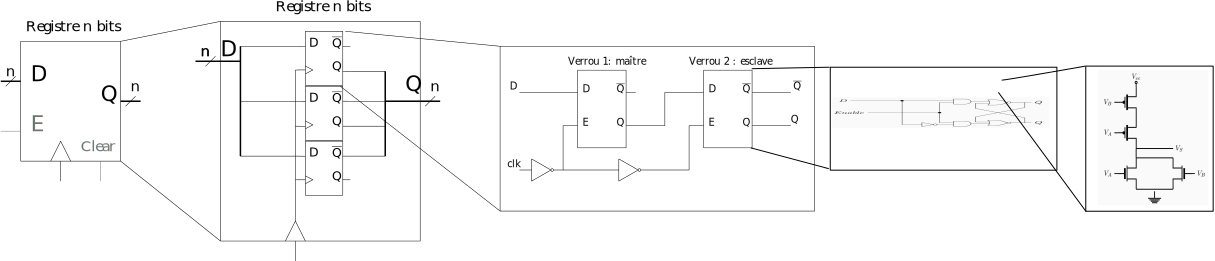
\includegraphics[width=\linewidth]{Figs/memory_register.pdf}
\end{block}

Capacité : $\approx$ 32-64 bits\\
Temps d'accès : $\approx$ 1 ps ($10^{-12}s$)\\
Volatile
\end{frame}

\begin{frame}
\frametitle{Les mémoires vives}
\begin{block}{Static Random Access Memory (SRAM)}
\centering\includegraphics[width=0.5\linewidth]{Figs/sram_inner.pdf}
\end{block}

Capacité : 10 Ko - 10 Mo\\
Temps d'accès : $\approx$ 1ns\\
Volatile
\end{frame}

\begin{frame}
\frametitle{Les mémoires vives}
\begin{block}{Dynamic random access memory (DRAM)}
\centering\includegraphics[width=0.4\linewidth]{Figs/dram_inner.pdf}
\end{block}

Capacité : 10 Go\\
Temps d'accès : 80 ns (réécriture toutes les ms)\\
Volatile
\end{frame}

\begin{frame}
\frametitle{Les mémoires de masse}
\begin{block}{Disque dur magnétique}
\centering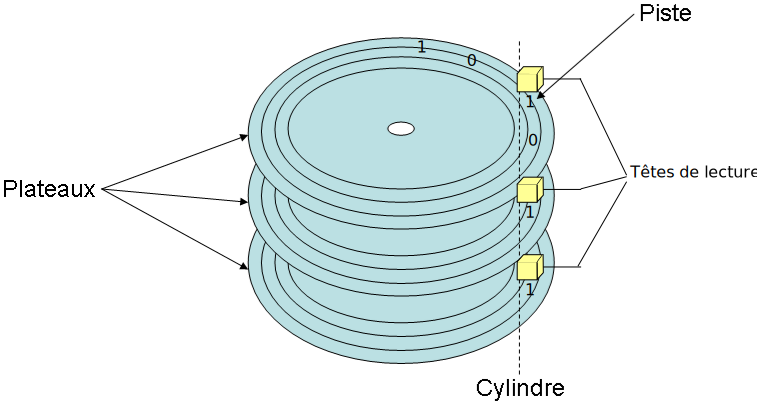
\includegraphics[width=0.5\linewidth]{Figs/dd.pdf}
\end{block}

Capacité : 1 To\\
Temps d'accès : 10 ms\\
Non volatile
\end{frame}

%% \begin{frame}
%% \frametitle{Les mémoires de masse}
%% \begin{block}{Disque dur SSD (Solide State Drive)}



%% \textcolor{red}{A faire !!}

%% \end{block}

%% Capacité : \\
%% Temps d'accès : \\
%% Non volatile
%% \end{frame}


\begin{frame}
\frametitle{Synthèse des mémoires vives et de masse}
\begin{block}{Compromis ?}
\begin{small}
\centering\begin{tabular}{cccc}
Type & Capacité & Latence & Coût (au  Gi-octet) \\
\hline
Registre & 100 bits & 20 ps & très cher\\
SRAM & 10 Ko - 10 Mo & 1-10 ns & $\approx$ 1000 \euro\\
DRAM & 10 Go & 80 ns & $\approx$ 10 \euro\\
\cline{2-3}
Flash & 100 Go & 100 $\mu s$& $\approx$ 1 \euro\\
%Disque dur SSD & 1 To & 1 ms & $\approx$ 0.5 \euro\\
Disque dur Magn & 1 To & 10 ms & $\approx$ 0.1 \euro
\end{tabular}
\end{small}
\end{block}
Une mémoire rapide et de grosse capacité ??
\end{frame}

\section{Mémoire cache}

\subsection{Principe de localité}

\begin{frame}
\frametitle{La clé}
\begin{block}{Les principes de localité}

\centering\includegraphics[width=0.5\linewidth]{Figs/localite.pdf}

\begin{itemize}
\item localité spatiale : les accès futures en RAM se feront à des addresses proches des accès courants
\item localité temporelle : une donnée accédée récemment sera certainement réutilisée prochainement
\end{itemize}
\end{block}
\end{frame}

\begin{frame}
\frametitle{Comment exploiter les principes de localité ?}
On combine :
\begin{enumerate}
\item une petite mémoire rapide avec 
\item une grosse mémoire lente
\end{enumerate}
Localité temporelle : on charge en mémoire rapide une donnée à laquelle on accède\\
Localité spatiale : on charge aussi les voisines\\
Politique de remplacement ? Dépends de la réalisation...
\end{frame}

\begin{frame}
\frametitle{Comment exploiter les principes de localité ?}

\begin{block}{Solution 1) A la charge du programmeur}

\centering\includegraphics[width=\linewidth]{Figs/nocache_mem}

\end{block}

$\rightarrow$ Pas très pratique...

\end{frame}


\begin{frame}
\frametitle{Comment exploiter les principes de localité ?}

\begin{block}{Solution 2) Hierarchie de mémoires}

\centering\includegraphics[width=\linewidth]{Figs/cache_mem}

\end{block}

\begin{block}{Performances du cache}

\begin{itemize}
\item Cache hit : la donnée est dans le cache $\Rightarrow$ accès rapide
\item Cache miss : la donnée n'est pas dans le cache $\Rightarrow$ accès lent
\end{itemize}
Hit ratio  : $\frac{hits}{hits+misses}$ \\
 Miss Ratio : $\frac{misses}{hits+misses}$\\
Temps moyen d'accès mémoire $T_m \approx HR. t_{cache} + MR. t_{mem}$\\
Pour $HR = 90\%$ : $T_m = 17 ns$.
\end{block}

\end{frame}

\subsection{Réalisation matérielle}

\begin{frame}
\frametitle{Principe de fonctionnement d'un cache}

\begin{block}{Principe}
A partir d'une petite information (clé), on retrouve le reste (valeur).\\
Analogie : annuaire téléphone
\end{block}

\begin{block}{En pratique}
L'adresse demandée est divisée en plusieurs parties dont une sert de clé.\\
Tableau associatif : Cache[clé] = \{adr, valeur, ...\}\\
Si la donnée est présente en cache : valide et accès rapide\\
Sinon il faut récupérer la donnée et la placer dans le cache.
\end{block}

\end{frame}

\begin{frame}
\frametitle{Réalisations matérielles d'un cache}
\begin{block}{Cache à correspondance directe}

\includegraphics[width=\linewidth]{Figs/direct_cache.pdf}

\end{block}
RAM[Adr] $\rightarrow$ Cache[Adr$_3$Adr$_2$Adr$_1$Adr$_0$]\\
pourquoi les bits de poids faibles comme index ?
\end{frame}

\begin{frame}
\frametitle{Réalisations matérielles d'un cache}
\begin{block}{Cache à correspondance directe par bloc}

\includegraphics[width=\linewidth]{Figs/direct_cache_block.pdf}

\end{block}

Un bloc : $2^{|offset|}$ mots;\\
Toutes les adresses de même ``Index'' ciblent la même ligne.
\end{frame}

\begin{frame}
\frametitle{Réalisations matérielles d'un cache}
\begin{block}{Cache associatif}

\centering\includegraphics[width=\linewidth]{Figs/associatif_cache.pdf}

\end{block}

Une donnée peut occuper n'importe quelle ligne de cache. Lourd matériellement.

\end{frame}


\begin{frame}
\frametitle{Réalisations matérielles d'un cache}
\begin{block}{Cache associatif à n entrées}

\centering\includegraphics[width=\linewidth]{Figs/nway_cache.pdf}

Indexable comme les caches directs, cache[index] étant associatif
\end{block}
\end{frame}

\subsection{Cohérence mémoire}

\begin{frame}
\frametitle{Cohérence cache/mémoire centrale}

\centering\includegraphics[width=\linewidth]{Figs/cache_mem}

\begin{block}{Problème}
Une donnée d'une \textbf{même adresse} peut être à la fois en \textbf{cache et} en \textbf{mémoire centrale.}
\end{block}

\begin{block}{Politiques d'écriture}
\begin{itemize}
\item Write through : propagation immédiate d'une modification vers la mémoire principale
\item Write back : écriture différée; écriture au remplacement (\emph{dirty bit})
\end{itemize}
\end{block}

\end{frame}


\section{Périphériques}

\begin{frame}
\begin{center}
\textbf{Les périphériques d'entrée/sortie}
\end{center}
\end{frame}

\subsection{Aperçu}

\begin{frame}
\frametitle{Les périphériques}

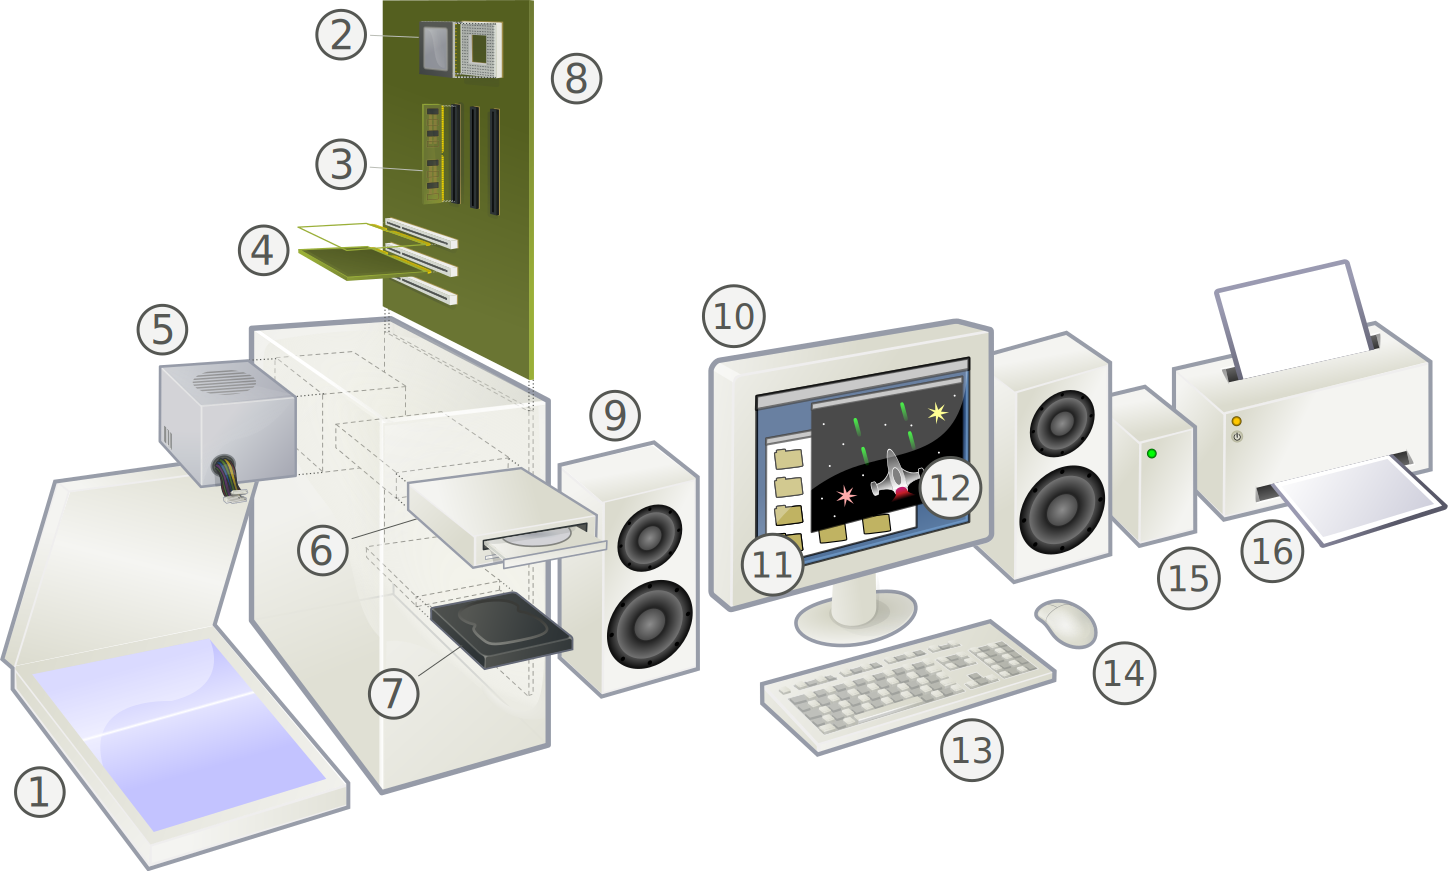
\includegraphics[width=\linewidth]{Figs/peripherique.pdf}


\begin{tiny}
http://www.wikipedia.org
\end{tiny}

\end{frame}


\begin{frame}
\frametitle{Structure d'un périphérique}

Au périphérique est associé un contrôleur (e.g. contrôleur disque) qui possède~:
\begin{itemize}
\item des registres 
\item des mémoires 
\item des machines à état 
\item ...
\end{itemize} 
Le périphérique est couplé aux bus d'adresses, données, contrôle.

\end{frame}

\subsection{Bus}

\begin{frame}

\frametitle{Interconnexion des périphériques et du chemin de données}

\includegraphics[width=\linewidth]{Figs/bus.pdf}

\end{frame}

\begin{frame}

\frametitle{Interconnexion des périphériques et du chemin de données}

\includegraphics[width=\linewidth]{Figs/chemin_peripherique.pdf}

\end{frame}

\begin{frame}

\frametitle{Interconnexion des périphériques et du chemin de données}

\includegraphics[width=\linewidth]{Figs/buses.pdf}

\begin{block}{Les bus}
\begin{small}
\begin{tabular}{ccccc}
Bus & Largeur (bits)  & Clk (MHz) & Débit (Mo/s)& Année\\
\hline
ISA 16 & 16  & 8.33 & 15.9 & 1984\\
PCI 32 & 32  & 33 & 125& 1993\\
AGP & 32	&66	&250 & 1997\\
PCI-E 3 (x16) & 16 & 8000 & 16000 & 2011
\end{tabular}
\end{small}
\end{block}

Bus parallèles (échange de mots, large mais court) / Bus série (bit à bit, e.g. USB)

\end{frame}


\begin{frame}
\frametitle{Comment contacter les entrées/sorties ?}

Il faut pouvoir contacter les registres du contrôleur du périphérique.

\begin{block}{E/S mappées en mémoire}

\begin{itemize}
\item comme pour un accès mémoire LDA, STA
\item avec des adresses réservées, ciblant les périphériques
\end{itemize}

\centering\includegraphics[width=0.5\linewidth]{Figs/io_mapped.png}

\end{block}

Autre solution : pas de bus d'adresse; placer dans le message un identifiant du destinataire.

\end{frame}


%% \begin{frame}
%% \frametitle{A mettre quelque part}
%% maitre/esclave\\
%% dma
%% \end{frame}







\subsection{Comment discuter sur le bus ?}

\begin{frame}

\frametitle{Protocoles d'échange : e.g. lecture mémoire}

\begin{block}{Echange synchrone}

\centering\includegraphics[width=0.7\linewidth]{Figs/true_sync_comm.pdf}

\end{block}

Fréquence d'horloge : ajustée au périphérique le plus lent

\end{frame}


\begin{frame}

\frametitle{Protocoles d'échange : e.g. lecture mémoire}

\begin{block}{Echange asynchrone : Master/Slave}

\centering\includegraphics[width=0.7\linewidth]{Figs/async_comm.pdf}

\end{block}

Pas d'horloge mais des signaux d'état : \emph{handshaking}\\
Plus réactif mais plus compliqué à mettre en oeuvre.

\end{frame}

\begin{frame}

\frametitle{Protocoles d'échange : e.g. lecture mémoire}

\begin{block}{Echange demi-synchrone}

\centering\includegraphics[width=0.7\linewidth]{Figs/sync_comm.pdf}

\end{block}

Attente ? e.g. Wait State : attente active

\end{frame}



%%\begin{frame}
%%\frametitle{Echange entre un périphérique et la mémoire centrale}

%% \begin{block}{}
%% \end{block}
%% \end{frame}

\begin{frame}
\frametitle{Et si on est plusieurs à vouloir parler ?}

On sait :
\begin{itemize}
\item comment interconnecter un périphérique avec le chemin de données : bus
\item comment réaliser un transfert synchrone/asynchrone
\end{itemize}
mais on a :
\begin{itemize}
\item ``un'' bus
\item plusieurs acteurs : mémoires, périphériques, CPU, ...
\end{itemize}

Nécessité d'arbitrer, e.g. le premier dans un certain ordre.\\

Et comment la demande d'échange du périphérique est prise en charge ?

\end{frame}

%% \begin{frame}
%% \frametitle{Direct Memory Access}
%% \end{frame}


\begin{frame}
\begin{center}
\textbf{Gestion des périphériques par interruption}
\end{center}
\end{frame}

\begin{frame}
\frametitle{Evènements synchrones}

Déroutements (\emph{trap}, \emph{exception}): événements synchrones avec l'exécution d'un programme, liés à une erreur : division par zéro, overflow, accès invalide à la mémoire : e.g. stack overflow

\begin{small}
\begin{block}{Ex : Overflow}
Comment prendre en charge des débordements lors d'opérations arithmétiques ?
\begin{enumerate}
\item le programme teste, après ``chaque'' opération, le bit \emph{overflow} (\emph{Status register})
\begin{itemize}
\item programme plus long en mémoire et à l'exécution et plus compliqué à écrire
\end{itemize}
\item dérouter le fil d'exécution si un débordement a lieu (à la JZA); \underline{pas de surcoût !}
\end{enumerate}
\end{block}
\end{small}

Au regard d'un programme, on peut prévoir quand un déroutement peut avoir lieu.
\end{frame}

\subsection{Interruptions}

\begin{frame}
\frametitle{Evènements asynchrones}

Evènements asynchrones; e.g. appui sur un bouton, une touche de clavier, bourrage papier, lecture mémoire terminée, ...
\begin{block}{Prise en charge par scrutation}
On interroge régulièrement le périphérique 
\begin{itemize}
\item programmation explicite
\item surcoût à l'exécution 
\end{itemize}
\end{block}
\begin{block}{Prise en charge par interruption}
Ecoute passive du périphérique : exécute un programme particulier que lorsque le périphérique lève une demande d'interruption\\
$\rightarrow$ sollicite moins le processeur (e.g. lecture sur disque : données prêtes)
\end{block}
\end{frame}

\begin{frame}
\frametitle{Modification du chemin de données}

On ajoute une ligne de requête d'interruption (INTR) qu'un périphérique peut mettre à l'état haut. Registre IF pour y être sensible ou non.

\includegraphics[width=\linewidth]{Figs/premier_chemin_seq_irq.pdf}

\end{frame}


\begin{frame}
\frametitle{Ecoute passive des demandes d'interruption}

Avant le fetch/decode, on test si une demande d'interruption est levée :
\begin{itemize}
\item sinon, on entre dans la phase de fetch/decode et exécution de l'instruction
\item si oui, on part en interruption
\end{itemize}

\begin{small}
\begin{tabular}{ccc|cl}
CodeMCount & Z & INTR \& IF & $S_1S_0$ & Sémantique\\
\hline
000 &  - & - & 00 & MicroPC := MicroPC+1\\
001 &  - & - & 01 & MicroPC := @Adr\\
010 &  - & - & 10 & MicroPC := Instruction\\
011 &  0 & - & 00 & MicroPC := MicroPC+1  si $S\neq 0$\\
011 &  1 & - & 01 & MicroPC := @Adr si $S=0$\\
100 &  - & 0 & 01 & MicroPC := @Adr si $\overline{INTR \& IF}$\\
100 &  - & 1 & 00 & MicroPC := MicroPC+1 si $INTR \& IF$
\end{tabular}
\end{small}

\end{frame}

%% \begin{frame}
%% \frametitle{Prise en charge de la demande d'interruption}

%% \includegraphics[width=\linewidth]{Figs/premier_chemin_seq_irq.pdf}

%% \end{frame}

\begin{frame}
\frametitle{Prise en charge de la demande d'interruption}

\begin{block}{Principe}
L'interruption doit être \textbf{gérée de manière transparente} pour le programme interrompu\\
$\Rightarrow$ sauvegarde du contexte d'exécution (sur la pile)
\end{block}

\begin{block}{Nouvelles instructions}
\begin{itemize}
\item INT (0xE000) : partir en interruption :
\begin{enumerate}
\item sauvegarde du contexte d'exécution sur la pile
\item chargement de l'adresse du programme d'interruption
\end{enumerate}
\item RTI (0xE800): revenir d'une interruption :
\begin{enumerate}
\item restauration du contexte d'exécution du programme interrompu
\end{enumerate}
\item STI (0xD400) : démasque les interruptions : IF := 1
\item CLI (0xD000) : Masque les interruptions : IF := 0
\end{itemize}
\end{block}

\end{frame}

\begin{frame}[fragile]
\frametitle{Comment savoir quel programme exécuter en cas d'interruptions}

Vecteur d'interruption : programme à exécuter en cas d'interruption\\
On stocke une table des vecteurs d'interruption en début de mémoire :

\begin{verbatim}
      JMP init
      JMP introutine
init: ... ; le programme principal
      ...

introutine: ... ; la routine d'interruption
            ...
            RTI ; le retour d'interruption
\end{verbatim}

\end{frame}

\begin{frame}
\frametitle{Chez nous : une seule interruption}

Nous ne prendrons ici en charge qu'une interruption, l'adresse de la routine d'interruption est codée en dur, dans le registre INTAdr

\centering\includegraphics[width=0.7\linewidth]{Figs/intadr.pdf}

\end{frame}

\begin{frame}
\frametitle{Résumons}

\begin{small}
\begin{enumerate}
\item le périphérique lève une requête d'interruption INTR=1
\item le processeur détecte la requête
\item le processeur accuse réception
\item le processeur sauvegarde l'état courant et se branche sur la routine d'interruption (vecteur d'interruption ou \emph{interrupt handler})
\item le processeur restaure l'état
\end{enumerate}
\end{small}

\centering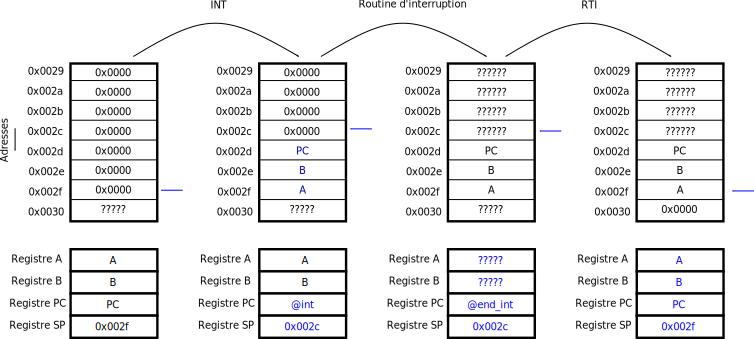
\includegraphics[width=0.7\linewidth]{Figs/irq.png}

\end{frame}

\begin{frame}
\frametitle{L'initialisation}

\begin{block}{Attention}
La gestion de l'interruption implique la pile !!\\
$\Rightarrow$ Phase d'initialisation (JMP init) minimale :
\begin{enumerate}
\item par défaut IF = 0
\item LDSPI ...
\item STI
\end{enumerate}
\end{block}

\end{frame}

\begin{frame}
\frametitle{Exemple jouet : \textcolor{red}{En BE}}

\includegraphics[width=\linewidth]{Figs/premier_chemin_seq_irq_bouton.pdf}

\end{frame}

\begin{frame}
\frametitle{Plusieurs interruptions ?}

On s'est limité pour le moment à un seul périphérique.
\begin{block}{Prise en charge de plusieurs interruptions}
\begin{enumerate}
\item Plusieurs lignes d'interruptions
\item Centralisation et arbitrage des demandes d'interruptions; Le vecteur d'interruption est récupéré sur le bus de données

\centering\includegraphics[width=0.6\linewidth]{Figs/8259.png}

\end{enumerate}
\end{block}
\end{frame}

\begin{frame}
\frametitle{Petits pas vers l'OS : Ordonnanceur}

\begin{block}{Problème}
Comment exécuter plusieurs programmes ``en même temps'' :
\begin{enumerate}
\item avec plusieurs chemins de données (architectures multi-coeurs)
\item avec un seul chemin de données partagé par deux programmes~: \textcolor{red}{en TL} 
\end{enumerate}
\end{block}

\end{frame}

\begin{frame}

\frametitle{Initialisation}

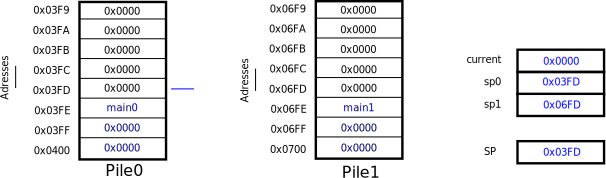
\includegraphics[width=\linewidth]{Figs/stack_ordonnanceur_init.png}

\end{frame}

\begin{frame}

\frametitle{Basculement de contexte}

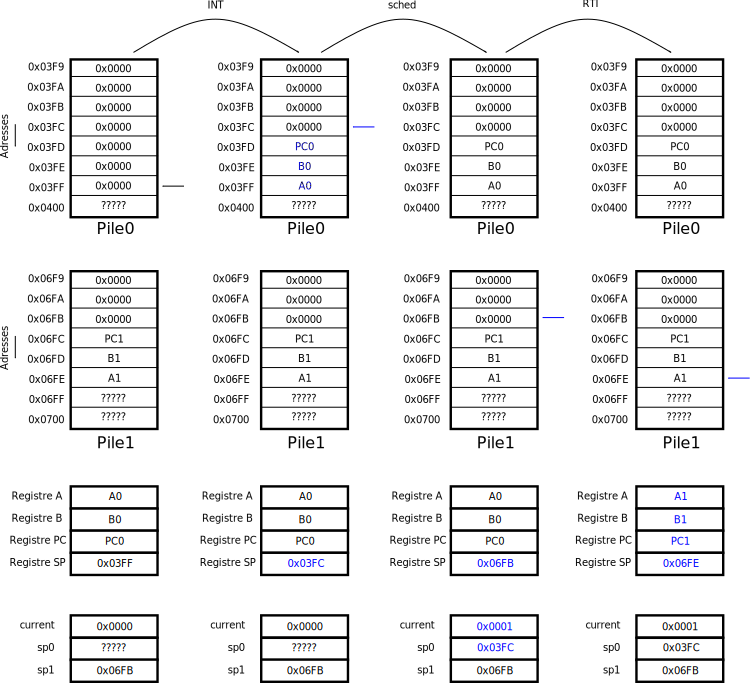
\includegraphics[width=\linewidth]{Figs/stack_ordonnanceur.png}

\end{frame}

%% \begin{frame}
%% \begin{center}
%% \textbf{Quantifier et améliorer les performances du chemin de données}
%% \end{center}
%% \end{frame}

%% \begin{frame}
%% \frametitle{Quantifions}

%% Latence et débit

%% % http://computationstructures.org/notes/performance/notes.html

%% \end{frame}

\begin{frame}
\begin{center}
\textbf{Rétrospective et conclusion}
\end{center}
\end{frame}

\begin{frame}
\frametitle{Cours 1 : Codons tout en binaire}
\begin{block}{Codage/décodage}

\centering\includegraphics[width=\linewidth]{Figs/synthese1.pdf}

\end{block}
\end{frame}

\begin{frame}
\frametitle{Cours 2-3 : Transistors, Circuits logiques, séquenceur}
\begin{block}{Couche physique}

\centering\includegraphics[width=0.1\linewidth]{Figs/circuits_mos.pdf}

$\Rightarrow$ Electronique analogique (ELAN), physique des semi-conducteurs
\end{block}
\begin{block}{Couche logique}

\centering\includegraphics[width=0.5\linewidth]{Figs/circuits_logique_combinatoire.pdf}

$\Rightarrow$ Systèmes logiques et électronique associée (SLEA)
\end{block}
\end{frame}

\begin{frame}
\frametitle{Cours 4-5 : pile et programmation}
\begin{block}{Pile et procédures}

\centering\includegraphics[width=0.5\linewidth]{Figs/respo_pile.pdf}

\end{block}
\begin{block}{Programmation}
$\Rightarrow$ Fondement de l'informatique et structures de données (FISDA)
\end{block}
\end{frame}

\begin{frame}
\frametitle{Cours 6 : mémoires caches}
\begin{block}{Hierarchie de mémoire}

\centering\includegraphics[width=0.6\linewidth]{Figs/localite.pdf}

\centering\includegraphics[width=\linewidth]{Figs/cache_mem}

\end{block}
\end{frame}

\begin{frame}
\frametitle{Cours 7 : périphériques et interruptions}

\includegraphics[width=\linewidth]{Figs/chemin_peripherique.pdf}

\end{frame}

\begin{frame}
\frametitle{Cours xx}
$\Rightarrow$ Systèmes d'informations (SI)
\begin{enumerate}
\item Systèmes d'exploitation :
\begin{itemize}
\item couche d'abstraction supplémentaire
\item systèmes de fichiers
\item mémoire virtuelle
\item ordonnanceur
\item ...
\end{itemize}
\item ......
\end{enumerate}
%\begin{itemize}
%\item architectures mono-coeur pipelinées
%\item architectures multi-coeurs
%\end{itemize}
\end{frame}
%% \begin{frame}
%% \frametitle{Principe du pipelining}
%% \end{frame}

%% \begin{frame}
%% \frametitle{Mise en oeuvre du pipelining}
%% \end{frame}

%% \begin{frame}
%% \frametitle{Prédiction de branchement}
%% \end{frame}

%% \begin{frame}
%% \frametitle{Architectures multi-coeurs}
%% \end{frame}



%% \section{Procédures, pile et pointeur de pile}
%% \section{Traduction, compilation, interprétation}
%% \section{Les mémoires}
%% \section{Les périphériques}
%% \section{Les interruptions}
%% \section{Suppléments}

%------------------------------------------------

%----------------------------------------------------------------------------------------

\end{document} 
